\section{Inference for Categorical Data: Proportions}

Often when we have a population and some sort of category that we can put them
into, we use samples to gain an estimate for the proportions of the population
as a whole. These give us estimates for the mean of the population, which we can then in turn use to find an estimate for the standard deviation of the population.

\begin{blackbox}
    \begin{definition}
        We define the \textbf{confidence interval} to be the interval of values
        from \( z^* \sigma \) below \( \hat{p} \) to \( z^* \sigma \) above \(
        \hat{p} \), where \( z^* \) is some number known as the
        \textbf{critical value}. This tells us that after repeated sampling,
        around \( 95\% \) (this is in the case of \( z^* = 2 \), in general
        this percent level is called the \textbf{confidence level}) of the
        time, the population mean will be contained in the interval.
    \end{definition}
\end{blackbox}

\begin{example}
    One often sees the confidence interval in the form \( \hat{p} \pm z^* \sigma \).
\end{example}

In order for us to make inferences on our populations, we must uphold the following rules:
\begin{enumerate}
    \item Samples are random.
    \item Samples are not skewed. This can be determined with the rule of thumb
        of \( 10 \) successes and \( 10 \) failures at least.
    \item Samples are (roughly) independent. A good way to determine this is
        the \( 10\% \) rule.
\end{enumerate}

\begin{blackbox}
    \begin{definition}
        A \textbf{null hypothesis} is a hypothesis that essentially states that
        "everything is as normal," and that what was assumed beforehand remains
        true after some change. An \textbf{alternate hypothesis} is one which
        counters this and says that something has changed after a change.
    \end{definition}
\end{blackbox}

When we want to find out whether changing something or doing something actually
affects a parameter in statistics, we set up a \textbf{significance test},
which contains:
\begin{itemize}
    \item Some sort of null hypothesis and alternate hypothesis that predict
        what will happen in response to the change. The null hypothesis says
        nothing will happen, while the alternate hypothesis says something will
        change.
    \item A sample. After conducting a test, we calculate the sample statistics.
    \item A \( p \)-value. After getting the sample statistics, we find the \(
        p \)-value, or probability that we could have gotten the results that
        we did given the null hypothesis being true.
    \item A significance level, denoted by \( \alpha \), which \textbf{is set
        before conducting the experiment}. After finding the \( p \)-value, we
        can compare it against our threshold \( \alpha \) to see whether the
        test impacted the statistics in a significant way or not. If \( p < a
        \), then we can reject the null hypothesis and say there was some
        effect. Otherwise, we do not reject the null hypothesis.
\end{itemize}

\begin{blackbox}
    \begin{definition}
        A \textbf{Type I error} is a false positive, in which the null
        hypothesis is true, yet we reject it anyway. A \textbf{Type II error}
        is a false negative, in which the null hypothesis is false but we fail
        to reject it.
    \end{definition}
\end{blackbox}

\begin{figure}[t]
    \centering
    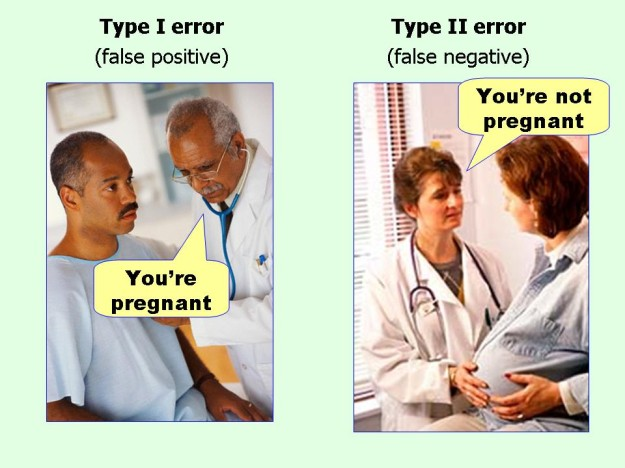
\includegraphics[scale=0.3]{type12error}
    \caption{An example displaying the difference between a Type I error and a Type II error.}
\end{figure}

When dealing with significance tests, we also have the notion of
\textbf{power}, or the probability that we reject the null hypothesis given
that it is false. We can increase this power by increasing \( \alpha \)
(although this comes at the cost of directly increasing the probability of a
Type I error) or by increasing sampling sizes. In general, lower variance and
higher distance between the null hypothesis and alternate hypothesis also lead
to higher power.

When doing a two-sample \( z \) test, remember that both samples do
\textbf{NOT} have to be necessarily the same size.
